\documentclass{beamer}
\usepackage{textcomp}
\usepackage{listings}
\usepackage{tikz}
\usetikzlibrary{shapes.geometric, arrows, positioning, shadows}
\tikzstyle{process} = [rectangle, minimum width=3cm, minimum height=1cm, text centered, text width=6cm, draw=black]
\tikzstyle{arrow} = [thick,->,>=stealth]
\lstset{ 
  backgroundcolor=\color{white},   % choose the background color; you must add \usepackage{color} or \usepackage{xcolor}; should come as last argument
  basicstyle=\footnotesize,        % the size of the fonts that are used for the code
  breakatwhitespace=false,         % sets if automatic breaks should only happen at whitespace
  breaklines=true,                 % sets automatic line breaking
  captionpos=b,                    % sets the caption-position to bottom
  commentstyle=\color{green},    % comment style
  escapeinside={\%*}{*)},          % if you want to add LaTeX within your code
  extendedchars=true,              % lets you use non-ASCII characters; for 8-bits encodings only, does not work with UTF-8
  frame=single,	                   % adds a frame around the code
  keepspaces=true,                 % keeps spaces in text, useful for keeping indentation of code (possibly needs columns=flexible)
  keywordstyle=\color{blue},       % keyword style
  language=Scala,                  % the language of the code
  numbers=none,                    % where to put the line-numbers; possible values are (none, left, right)
  rulecolor=\color{black},         % if not set, the frame-color may be changed on line-breaks within not-black text (e.g. comments (green here))
  showspaces=false,                % show spaces everywhere adding particular underscores; it overrides 'showstringspaces'
  showstringspaces=false,          % underline spaces within strings only
  showtabs=false,                  % show tabs within strings adding particular underscores
  stepnumber=2,                    % the step between two line-numbers. If it's 1, each line will be numbered
  stringstyle=\color{purple},     % string literal style
  tabsize=2,	                   % sets default tabsize to 2 spaces
  title=\lstname                   % show the filename of files included with \lstinputlisting; also try caption instead of title
}
\usepackage[utf8]{inputenc}
%\usetheme{CambridgeUS}
%\usefonttheme{professionalfonts}
\usecolortheme{beaver}
 
%Information to be included in the title page:
\title{Tastydoc}
\subtitle{A documentation tool for dotty using TASTy files}
\author{Bryan Abate}
\date{19th June 2019} 
 
\begin{document}
 
\frame{\titlepage}

\AtBeginSection[]
{
  \begin{frame}
    \frametitle{Table of Contents}
    \tableofcontents[currentsection]
  \end{frame}
}

\section{Introduction}

\begin{frame}
\frametitle{What is Tastydoc ?}
\begin{itemize}
  \item Documentation tool for Dotty \pause
  \item Uses TASTy files \pause
  \item Outputs Markdown
\end{itemize}
\end{frame}
 
\section{Features}

\begin{frame}
  \frametitle{Accessible information}
  \begin{itemize}
    \item Annotations, modifiers (including scope modifiers), parameters, type parameters, and return types \pause
    \item Members, parents, constructors, known subclasses and companion \pause
    \item User documentation (Wiki-style \& Markdown)
  \end{itemize}
\end{frame}

\begin{frame}
  \frametitle{TASTy}
  \begin{itemize}
    \item Extract information from them \pause
    \item Independent from the compiler
  \end{itemize}
\end{frame}

\begin{frame}
  \frametitle{Linking}
  \begin{itemize}
    \item To types \pause
    \item Companion \pause
    \item Annotations \pause
    \item Scope modifiers \pause
    \item Parents
  \end{itemize}
\end{frame}

\begin{frame}
  \frametitle{Markdown}
  \begin{itemize}
    \item Easy to edit by hand \& preview \pause
    \item Easy to add own files \pause
    \item Easy for the user to make links \pause
    \item Git hosting service have built-in preview \pause
    \item Easy to convert to another format (HTML, PDF, etc.)
  \end{itemize}
\end{frame}

\section{Architecture}

\begin{frame}
  \frametitle{Representation}
  \begin{itemize}
    \item Contain information about an entity \pause
    \item Easy to use, no knowledge of TASTy required \pause
    \item Code is easy to maintain \pause
    \item Similar to Dottydoc Entity \textrightarrow can reuse Dottydoc code
  \end{itemize}
\end{frame}

\begin{frame}
  \frametitle{Reference}
  \begin{itemize}
    \item Contain information about types \pause
    \item Necessary for linking \pause
    \item Inspired by Dottydoc
  \end{itemize}
\end{frame}

\begin{frame}[fragile]
  \frametitle{User documentation}
  \begin{itemize}
    \item Access to all @ except \texttt{@usecase} and \texttt{@define}\pause
    \item Support Wiki-style and Markdown \pause
    \item Uses Dottydoc code modified for:
    \begin{itemize}
      \item Markdown output
      \item Small changes in structure 
    \end{itemize}
  \end{itemize}
\end{frame}

\begin{frame}
  \frametitle{Workflow}
  \begin{center}
    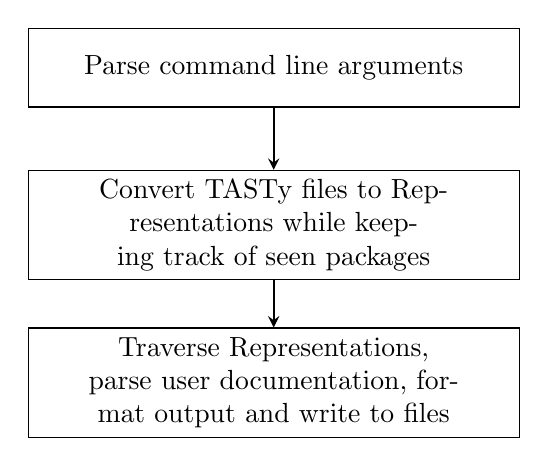
\begin{tikzpicture}[node distance=2cm]
        \node (parse) [process] {Parse command line arguments};\pause
        \node (convert) [process, below of=parse] {Convert TASTy files to Representations while keeping track of seen packages};
        \draw [arrow] (parse) -- (convert);\pause
        \node (output) [process, below of=convert] {Traverse Representations, parse user documentation, format output and write to files};
    
        \draw [arrow] (convert) -- (output);
    \end{tikzpicture}
  \end{center}
\end{frame}

\section{Dottydoc vs Tastydoc}

\begin{frame}
  \frametitle{General comparison}
  \begin{itemize}
    \item Compiler internals \pause
    \item Markdown vs HTML/CSS
  \end{itemize}
\end{frame}

\begin{frame}
  \frametitle{Extra features}
  \begin{itemize}
    \item Scope modifiers \pause
    \item Known subclasses \pause
    \item Refined types
  \end{itemize}
\end{frame}

\begin{frame}[fragile]
  \frametitle{Bugs fixed}
  \begin{itemize}
    \item Buggy output
\begin{lstlisting}
final val BITS_PER_LAZY_VAL : [31m2L[0m
\end{lstlisting}\pause
    \item Wrong parents \pause
    \item Annotations \pause
    \item Compiler artifacts \pause
    \item potentially program breaking code
\begin{lstlisting}[language=scala]
def parents: List[Entity] = this :: this.parents
\end{lstlisting}
  \end{itemize}
\end{frame}

\section{Problems \& Further work}

\begin{frame}
  \frametitle{Problems}
  \begin{itemize}
    \item Markdown escaping \pause
    \item Linking inside code blocks \pause
    \item Section \pause
    \item IDs for linking
  \end{itemize}
\end{frame}

\begin{frame}[fragile]
  \frametitle{Further work}
  \begin{itemize}
    \item Markdown escaping \pause
    \item Type lambdas \pause
    \item Complex types
\begin{lstlisting}[language=scala]
  class Graph {
      type Node = Int
  }
  def linkingGraph(g: Graph): g.Node = ???    
\end{lstlisting}\pause
    \item Default values \pause
    \item Extra user-documentation parsing \pause
    \item HTML/CSS
  \end{itemize}
\end{frame}

\end{document}